\documentclass[a4paper, 11pt]{article}
\usepackage{graphicx}
\usepackage[frenchb]{babel}
\usepackage[utf8]{inputenc}
\title{Rapport de la Zboobteam}
\author{Boisson Pacien - Sarlin Nicolas - Taton Sven}
\date{Vendredi 14 Décembre 2012} 

%Début du rapport
\begin{document}
\maketitle
\tableofcontents
\newpage
\section{Introduction}
Le projet consiste à réaliser une base de données contenant les informations nécéssaires à l'organisation d'un foyer étudiant.\\
Le foyer étudiant organise des évènements pour les élèves, au cours desquels ces derniers utilisent des jeux, il serait utile de conserver un historique des évènements organisés et des jeux utilisés pour l'occasion. Le foyer est aussi une bibliothèque associative, les élèves pouvant y emprunter des livres, il serait donc aussi utile de conserver un historique des emprunts de livres.
\newpage
\part{Modélisation des données}
\setcounter{section}{0}
\section{Description du contexte de l'application}
Tous les élèves de l'école sont des utilisateurs du foyer, chaque élève est caractérisé par l'année à laquelle il quittera l'école, sa promo. Parmi ces élèves, certains sont ou ont été membres du bureau, donc administrateurs du foyer pendant une année. Le foyer organise des évènements ponctuels dans divers lieux, au cours desquels il utilise un ou plusieurs jeux, et auxquels les élèves peuvent participer. Un livre donné est disponible en un ou plusieurs exemplaires au foyer, ces livres peuvent être empruntés par les élèves.
\section{Modèle entité-association}
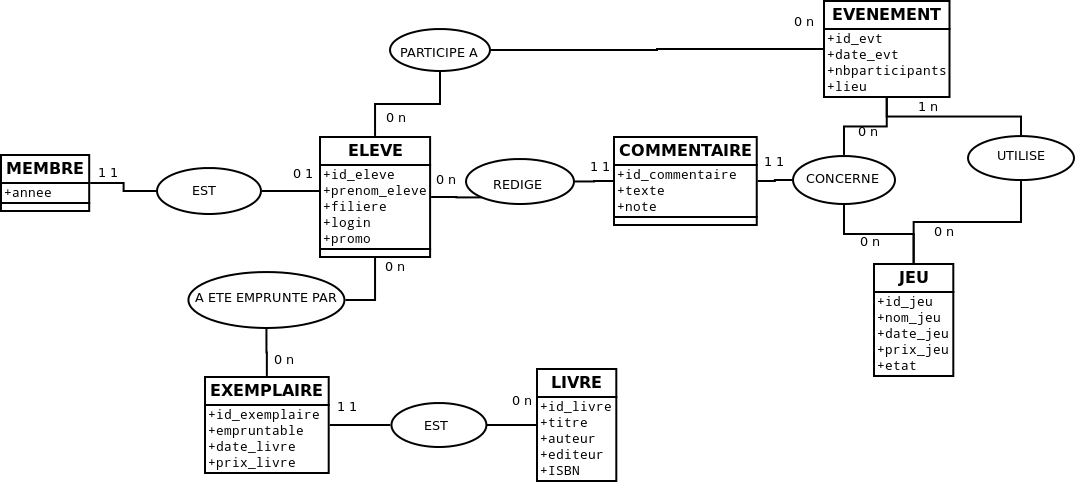
\includegraphics[width=1.2\textwidth]{ER.png}
Les conventions de nommage utilisées sont les suivantes : Les noms d'entité/association sont écrits en majuscule. Les clés sont en minuscule. En cas d'ambigu\"ité entre deux noms, on rajoute un symbole \_, suivi du nom de la table en minuscule. Les clés primaires commencent par id.
\paragraph{}
Les entités sont celles demandées dans le sujet, à l'exception de l'entité EXEMPLAIRE. Celle ci a été créée pour distinguer le livre au sens virtuel (qui possède titre, auteur, editeur et ISBN) de l'objet physique. Ainsi, un élève emprunte un exemplaire et non pas un livre. Nous avons aussi choisi de réaliser une association A ETE EMPRUNTE PAR (emprunts actuels et passés plut\^ot que EST EMPRUNTE PAR afin de pouvoir conserver l'historique des emprunts (utile pour les requ\^etes de statistiques).\\
Nous considérons aussi que lorsque le sujet mentionne l'action pour un élève de lire un livre, il s'agit en fait de l'emprunter (on n'enregistre pas dans la base de donnée à chaque fois qu'un élève consulte un livre sur place). 
\section{Liste des opérations prévues sur la base}
\subsection{Opérations sur les membres du bureau}
\begin{itemize}
\item Obtenir un historique complet des membres du bureau, ou obtenir la liste des membres du bureau pendant une année donnée.
\item Obtenir la liste des membres du bureau qui ont participé à un évènement après avoir effectué leur mandat.
\item Ajouter, supprimer, modifier des membres du bureau
\end{itemize}
\subsection{Opérations sur les élèves}
\begin{itemize}
\item Obtenir les informations (nom, prénom, promo, login) d'un élève donné.
\item Ajouter, supprimer, modifier des élèves.
\end{itemize}
\subsection{Opérations sur les évènements}
\begin{itemize}
\item Obtenir la liste des évènements auquels a participé un membre pendant une année donnée.
\item Obtenir la liste des participants à un évènement donné.
\item Ajouter, supprimer, modifier des évènements.
\end{itemize}
\subsection{Opérations sur les livres}
\begin{itemize}
\item Obtenir la liste des emprunts par élève pour un livre donné.
\item Obtenir la moyenne des emprunts par mois sur une année.
\item Obtenir le classement des livres les plus lus.
\item Ajouter, supprimer, modifier des membres des livres et des exemplaires.
\end{itemize}
\subsection{Opérations sur les jeux}
\begin{itemize}
\item Obtenir la liste des jeux utilisés pour un évènement donné.
\item Obtenir le classement des jeux réalisant le plus d'inscriptions aux évènements où ils sont utilisés.
\item Ajouter, supprimer, modifier des jeux
\end{itemize}
\newpage
\part{Schéma relationnel}
\setcounter{section}{0}
\section{Passage au relationnel}
Le passage au modèle relationnel nécessite d'étudier les particularités de chaque association pour créer les bonnes relations. Certaines nécessitent la création de nouvelles tables, d'autres se contentent d'un ajout de clé étrangère.
\section{Contraintes d'intégrité et dépendances fonctionnelles}
\section{Schéma relationnel en $3^{eme}$ forme normale}
\newpage
\part{Implantation}
\setcounter{section}{0}
\section{Création de la base de données}
\section{Implémentation des commandes SQL}
\newpage
\part{Utilisation}
\setcounter{section}{0}
\section{Description de l'environnement d'exécution}
\section{Notice d'utilisation}
\section{Description des interfaces éventuelles}
\end{document}
